%%
%% Author: darshan
%% 12/03/18
%%

% Preamble
\subsection{Frontend}
The requirement to have Frontend according to the usecase was questionable, but the system being able to provide the error detection and also monitoring of the system emphasized us to have user interactive application for monitoring, error identification and also provenance system data visualization. Thus, we developed an tailored frontend system satisfying actors like system administrator, analysts, developers, etc. Frontend represents the client-tier from the three-tier architecture. Its a loosely coupled service from the system giving enhanced security to the security and scalability.

\begin{figure}
    \centering
    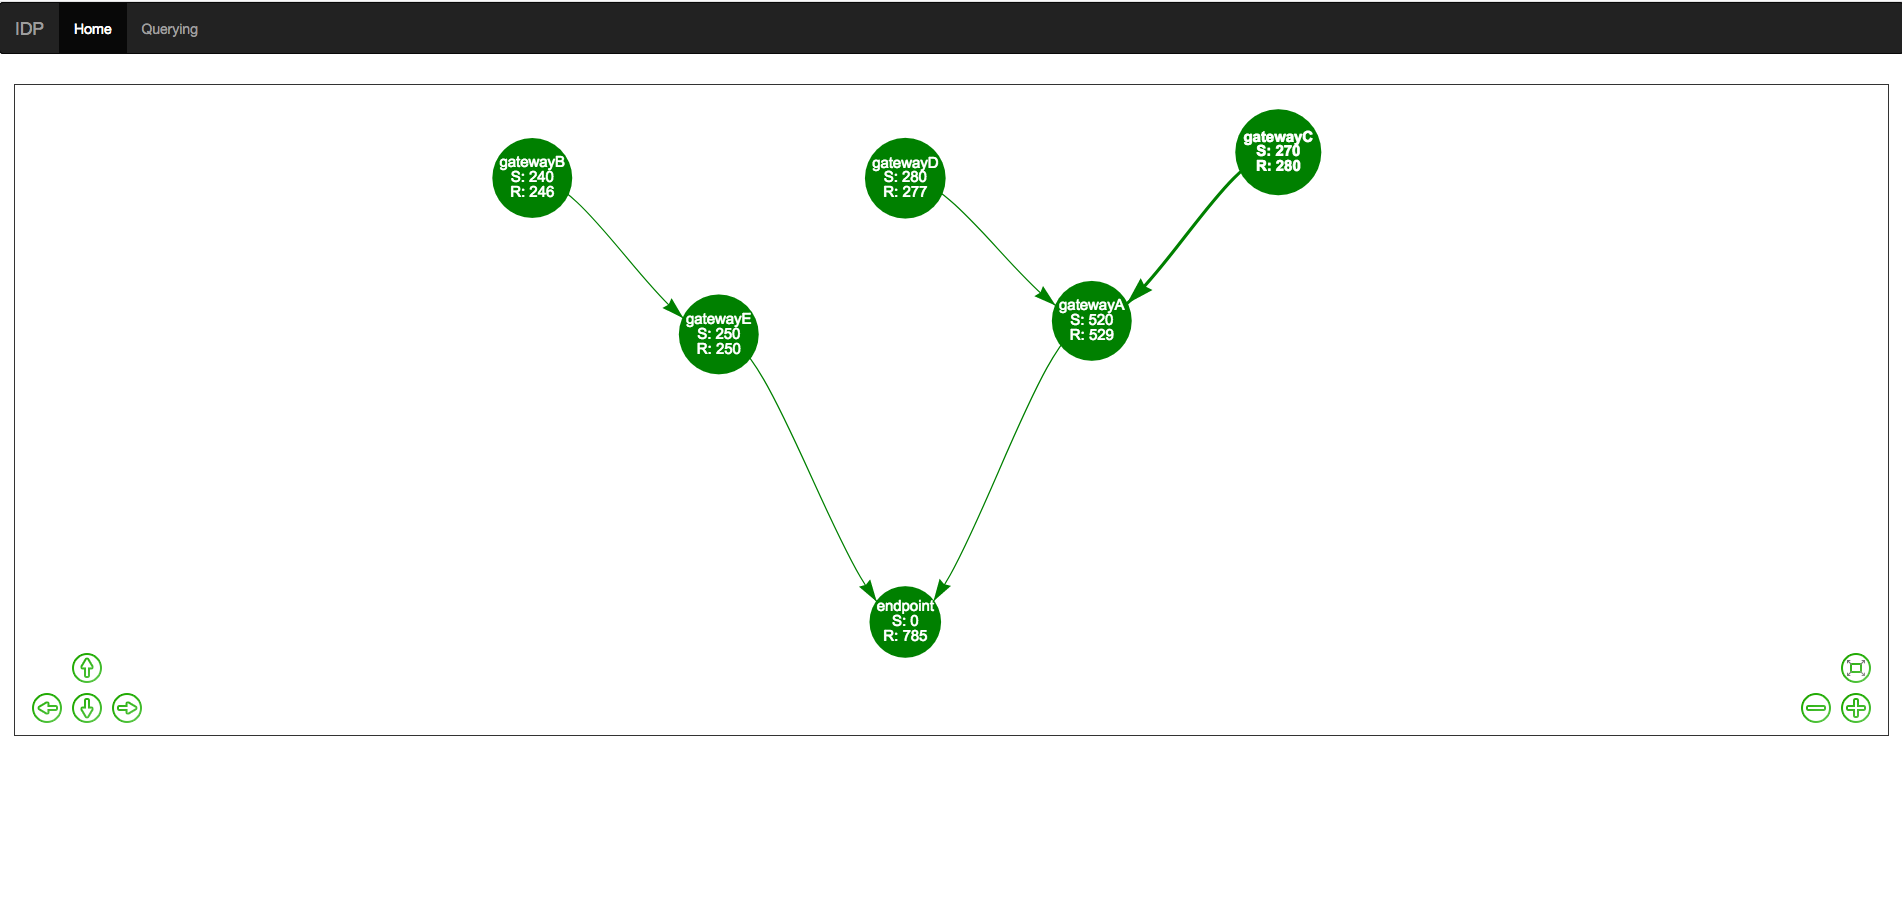
\includegraphics[width=\textwidth,height=10cm,keepaspectratio]{figures/dashboard.png}
    \caption{\label{fig:dashboard}Dashboard}
\end{figure}

The frontend application gives user a very interactive dashboard. The above figure \ref{fig:dashboard} shows Dashboard page when the end user access the system. The dashboard is very informative and helps the user to visualize the components in the provenance system pipeline. It gives a detail view of nodes and all related information about that node.

\subsubsection{Technology Used}

The frontend was developed with in-demand market technology like Javascript scripting language, Node.js, Express framework.

\begin{description}
    \item[Javascript] It was originally named Mocha is a “multi-paradigm language, supporting object-oriented, imperative, and functional programming styles.” \cite{javascript} JavaScript started on web browsers as language to dynamically interact with the user and control the components of the page. JavaScript’s language architecture is quite unique from other languages which is especially handy when developing web application that rely on non-blocking operation.
    \newline
    \newline
    JavaScript architecture combines object-oriented, functional and scripting languages paradigms. Syntax wise, JavaScript is based on C’s structured layout, with subroutines, block structures and loops. While it is object
    -oriented, JavaScript does not have classes, but instead
    rely on object prototypes for inheritance. This means that the methods and fields of the objects’ prototypes may be dynamically changed for future construction of these objects. Functions in JavaScript are also objects, and can be sent as arguments to other functions as the case in
    functional languages; functions can also have methods and properties of their own. JavaScript also provides dynamic typing as well as static typing. Variables could be defined with a specific type such as Number of String, or casted dynamically by initializing it as a var. Moreover, JavaScript, like scripting languages, allows the use of variadic functions (number of arguments is not defined), and supports Regular expressions such as in Perl. Finally, JavaScript’s support for associative arrays is the basis for the construction of JSON data formats. Using a single language throughout the stack enables the reuse of resources such as JSON objects which can be manipulated the same way by any part of the stack.
    \newline
    \newline
    There were several attempts aiming to place JavaScript on the server side ever since the mid-1990s. But, none of these solutions were as successful as Node.js which is pioneering a new way of server programming focused mainly around asynchronous operations. There are three
    main reasons that made JavaScript the language of choice of Node.js
    \begin{enumerate}
        \item Google’s V8 is an open-sourced high-performance JavaScript execution engine built for Chrome. It complies JavaScript to native machine code instead of interpreting it in real time. V8 and other JavaScript runtime engines also provide a concurrency model using a message queue and an event-loop which allows JavaScript to stack operations and their callbacks and execute the callback when the operation is done.
        \item JavaScript is built around an event-driven interaction model because it depends on user actions, which makes asynchronous, non-blocking and callbacks natural, as they are event driven as well.
        \item JavaScript is an interpreted language which makes it platform independent.
        \item JSON (
        JavaScript Object Notation). JavaScript has been the language of choice to control the web for a long time; and since the old days, data had to be marshelled into JSON
        objects when sent to the web. Because of the high dependence on JSON objects, a new 7 kind of JSON like databases were created, enabling the easy exchange of data between back-end and front-end.
    \end{enumerate}
    \item[Node.js] Node JS is a JavaScript platform for building fast, scalable, network applications built on
    Google’s V8 Engine. Node is single threaded and built around the paradigm of none-blocking IO. With Node.js each incoming request by the user is handled by one single thread in opposition to the multi-threaded techniques used by PHP to scale the operations. Each request handled by
    this thread is coupled with a callback function that is called upon completion of the task. This is possible due to the fundamental support of JavaScript for events, Asynchronous operations, and callbacks; and Node.js puts JavaScript on the server side. Node has several advantag
    es, some of which are:
    \begin{itemize}
        \item RESTful API. As Node can build an HTTP server out of the box, it can communicate with all other components through HTTP methods for CRUD operations based on the
        RESTful paradigm.
        \item Single Threaded. Since it is not blocking I/O operat
        ions, Node can handle all user requests using a single thread, instead of allocation of new thread for each request, which has a large memory footprint. Nonetheless, Node does use a thread pool at the kernel level to guarantee that the operations are being executed asynchronously without blocking the event-loop. This is necessary because the kernel does not support all operations asynchronously.
    \end{itemize}
    \item[NPM] he Node Package Manager is based on JavaScript's npm. A built-in module that supports package management, it can be used to easily download and install modules for a Node application. Moreover, Node already has many packages and libraries developed to work on top of it; all of which confine to the asynchronous nature of Node.js.
    \item[Express] Express is a fast, un-opinionated, minimalist web application framework for Node.js. It is designed for building web applications and is the de facto standard server framework for Node.js. Early 2016 the Express.js project was brought into the Node.js foundation as an incubating project. Express was itself a project in node generation which was split into three Github organizations called expressjs, pillarjs and jshttp. Express is a simple routing plus a sugar layer built on top of the actual base Node.js HTTP server that helps manage a server and the routes. It gives declarative routing without making s witch statements or i f statements or big functions, into a basic middleware pattern. \cite{express}
    \newline
    \newline
    One should already be familiar with JavaScript syntax and have Node.js installed to get started. There are many reasons why Express and Node are great choice for server side development.One major reason is that since Express is built on top of Node it is the perfect framework for ultra-fast input and output. Node.js is both asynchronous and single threaded- many requests can be made simultaneously without incurring of bottleneck that would slow down processing. The robust API that ships with express allows us to easily configure routes to send and receive
    requests from a front-end and connect to a database. \cite{express}
    \item[Bootstrap Styling Framework] This  framework  has  become  one  of  the  mo
    st  popular  framework  and  used  by  popular website. This framework is  a  lightweight  and  modular  front-end  framework  \cite{bootstrap}.   It  provides  a powerful  web  interfaces for a fast development.
    \item[Vis.js] A dynamic, browser based visualization library. The library is designed to be easy to use, to handle large amounts of dynamic data, and to enable manipulation of and interaction with the data. This library enabled use to visualize the nodes in the pipeline. and it was represented as DAG (Directed Arrow Graph). This library is licenses under Apache 4.0 and MIT \cite{visjs}.
\end{description}

\subsubsection{Design}
In this section we would discuss the design of the frontend. We used bootstrap with handlebars as our main UI design kit. Pug is a very powerful templating framework, alongside with bootstrap it gives a lot of flexibility with design. The styling and the javascript component integration made it the best choice for us to use it in our project. Bootstraps modular structure and less complicated stylesheet function, made it quite simpler for us to work on. Below are the list of pages and its corresponding functionalities: \ref{fig:dashboard}

\begin{itemize}
    \item \textbf{Home Page}: All the nodes are visualize in network topology using DAG (Directed-Arrow-Graph). Each node in the topology is has a predecessor and a successor node. The nodes in the topology shows relevant information for that particulate node and its running status. The nodes are represented as a circular design which encapsulate further details of the node. When user clicks on one of the nodes it shows last 50 provenance data generated in a tabular form. Navigation bar in home page only
    shows two options (i) Home (ii)Querying
    \item \textbf{HomePage/Node Click}: Clicking on a particular node with retrieve last 50 provenance data points generated during provenance capture.
    \item \textbf{HomePage/Visualize Provenance Lineage}: When the user performs click action on the button, it redirects user to a new page where the provenance data is plotted as a DAG(Directed-Arrow-Graph) along with all relevant context information.
    \item \textbf{Querying}: This page displays an `cql' editor which is a Cassandra Query script where an analyst or an system administrator can write queries to our Provenance Database according to his needs. The result are visualized in 2 forms (i) A tabular form (ii) JSON format.
    \item \textbf{Querying/Submit Query}: Once the end-user writes the query in the cql editor and presses the Submit button, then user is presented with the query result in the form of table.
    \item \textbf{Querying/JSON Query}: Once the end-user writes the query in the cql editor and presses the Submit JSON button, then user is presented with the query result in the form of JSON format.
\end{itemize}

\begin{figure}
    \centering
    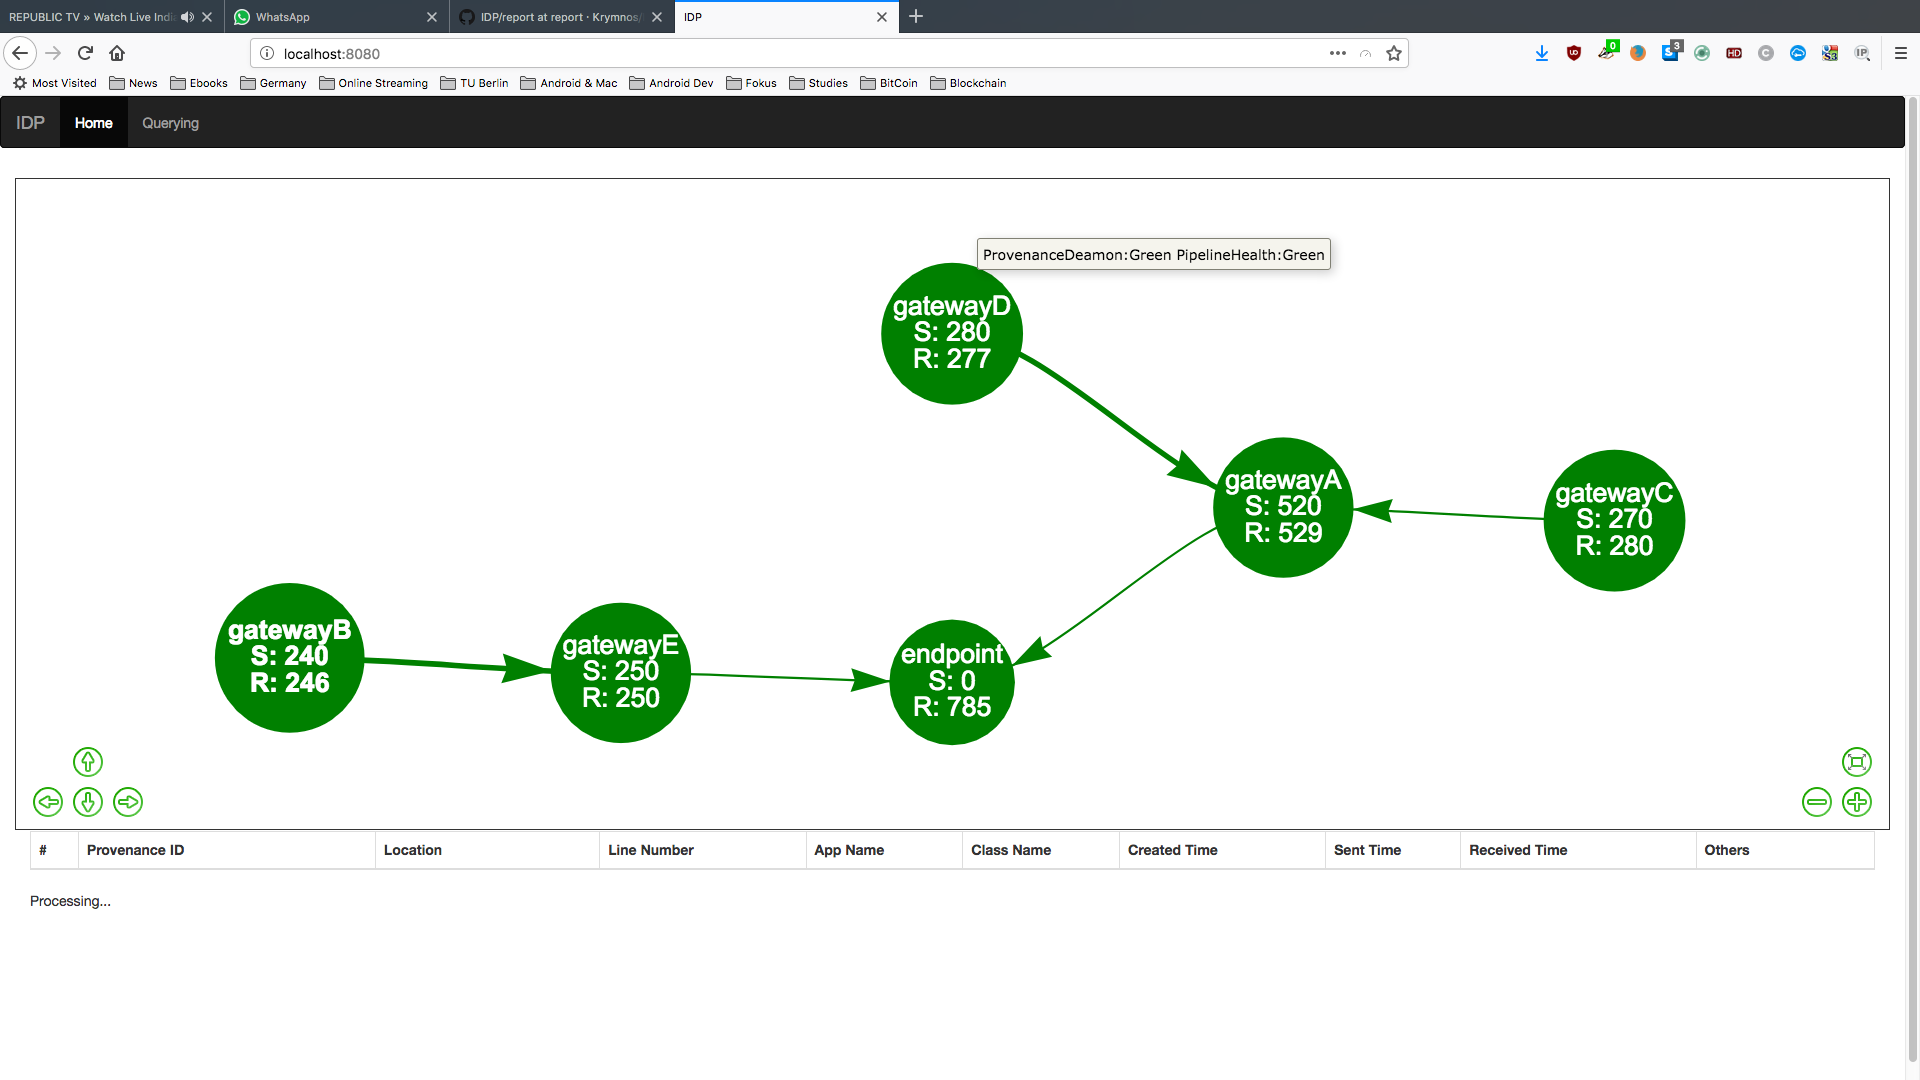
\includegraphics[width=\textwidth,height=10cm,keepaspectratio]{figures/node_visualization.png}
    \caption{\label{fig:nodes}Node Topology Visualization}
\end{figure}

\textbf{Node Visualization} In the figure \ref{fig:nodes}, it shows visualization of the nodes in the form of network topology in our  Smart-Grid system. The node defines many relevant information like its preceding and succeeding nodes. The inward arrow to the node defines its preceding node and the outward arrow from that node shows the succeeding node. Each node visualize in the circular form, and encapsulates node details like:
\begin{enumerate}
    \item node name,
    \item message send rate,
    \item message receive rate.
\end{enumerate}
Nodes are further more defined by colors. Node colors can be of 2 types (i) Green and (ii) Red. The Green color of the node denotes the health of the node which means the node is working as it should be. Red color denotes that the particular node is not working which helps the end user to come to a conclusion that there are some issues with node and its not working as it it supposed to. The directed edges also denotes by the color Green and Red. It shows the status of Pipeline Health giving further more granular detail about error in the pipeline system.
\newline
Many action can be performed on the node visualization. On clicking of particular node it further retrieves provenance data that were generated. The provenance data is displayed in the form of table with all context information like Provenance Id, Location, ClassName, LineNo etc. The table houses 3 buttons, (i) Visualizing the provenance data generated along the pipeline, (ii) downloading the provenance lineage in JSON format, (iii) downloading provenance data recursively in JSON format.
\newline
Further on clicking on the Visualize Provenance data button, a the control redirects to a new page which visualizes the provenance data across the pipeline and showing all relevant context parameters generated during provenance data capture.
